% ============================================
% model_template_setup.tex
% ============================================
% Defines \SetupModelTemplate{ModelWord} macro
% Maps generic template commands (\M...) to model-specific commands (\ModelX...)
%
% Usage in model chapters:
%   \SetupModelTemplate{One}   % For Model 1
%   \SetupModelTemplate{Two}   % For Model 2
%   \SetupModelTemplate{Five}  % For Model 5
%   etc.
%
% After calling this macro, the template can use generic commands like:
%   \MRSquaredTest   → maps to \ModelOneRSquaredTest (for Model 1)
%   \MRMSETest       → maps to \ModelOneRMSETest (for Model 1)
%   etc.
% ============================================
% Usage Example:
% ============================================
% In 3Alternative-1-CurrentUpdated.tex (Model 1):
%
% \chapter{Model 1: Re-evaluation of Model 5b}
% % Model 1 Calibrated Values
% Generated: 2025-10-02 01:58:23.185499
% Model: Linear with Outlier Removal

% Core Metrics
\renewcommand{\ModelOneRSquaredTrain}{0.2383}
\renewcommand{\ModelOneRSquaredTest}{0.2178}
\renewcommand{\ModelOneRMSETrain}{39,238}
\renewcommand{\ModelOneRMSETest}{39,500}
\renewcommand{\ModelOneMAETrain}{27,831}
\renewcommand{\ModelOneMAETest}{27,912}
\renewcommand{\ModelOneMAPETrain}{85.2}
\renewcommand{\ModelOneMAPETest}{84.8}
\renewcommand{\ModelOneCVMean}{0.2372}
\renewcommand{\ModelOneCVStd}{0.0196}
\renewcommand{\ModelOneWithinOneK}{2.4}
\renewcommand{\ModelOneWithinTwoK}{4.9}
\renewcommand{\ModelOneWithinFiveK}{15.8}
\renewcommand{\ModelOneWithinTenK}{28.5}
\renewcommand{\ModelOneWithinTwentyK}{49.5}
\renewcommand{\ModelOneTrainingSamples}{27,339}
\renewcommand{\ModelOneTestSamples}{6,834}

% Subgroup Metrics
\renewcommand{\ModelOneSubgrouplivingFHN}{5,941}
\renewcommand{\ModelOneSubgrouplivingFHRSquared}{0.222}
\renewcommand{\ModelOneSubgrouplivingFHRMSE}{39,928}
\renewcommand{\ModelOneSubgrouplivingFHBias}{-7,487}
\renewcommand{\ModelOneSubgrouplivingILSLN}{893}
\renewcommand{\ModelOneSubgrouplivingILSLRSquared}{0.179}
\renewcommand{\ModelOneSubgrouplivingILSLRMSE}{36,524}
\renewcommand{\ModelOneSubgrouplivingILSLBias}{-3,272}
\renewcommand{\ModelOneSubgroupageAgeUnderTwentyOneN}{694}
\renewcommand{\ModelOneSubgroupageAgeUnderTwentyOneRSquared}{0.138}
\renewcommand{\ModelOneSubgroupageAgeUnderTwentyOneRMSE}{34,649}
\renewcommand{\ModelOneSubgroupageAgeUnderTwentyOneBias}{-8,152}
\renewcommand{\ModelOneSubgroupageAgeTwentyOneToThirtyN}{1,797}
\renewcommand{\ModelOneSubgroupageAgeTwentyOneToThirtyRSquared}{0.161}
\renewcommand{\ModelOneSubgroupageAgeTwentyOneToThirtyRMSE}{44,751}
\renewcommand{\ModelOneSubgroupageAgeTwentyOneToThirtyBias}{-7,785}
\renewcommand{\ModelOneSubgroupageAgeThirtyOnePlusN}{4,343}
\renewcommand{\ModelOneSubgroupageAgeThirtyOnePlusRSquared}{0.218}
\renewcommand{\ModelOneSubgroupageAgeThirtyOnePlusRMSE}{37,876}
\renewcommand{\ModelOneSubgroupageAgeThirtyOnePlusBias}{-6,391}
\renewcommand{\ModelOneSubgroupcostQOneLowN}{1,709}
\renewcommand{\ModelOneSubgroupcostQOneLowRSquared}{-10.000}
\renewcommand{\ModelOneSubgroupcostQOneLowRMSE}{31,272}
\renewcommand{\ModelOneSubgroupcostQOneLowBias}{+24,162}
\renewcommand{\ModelOneSubgroupcostQTwoN}{1,708}
\renewcommand{\ModelOneSubgroupcostQTwoRSquared}{-6.029}
\renewcommand{\ModelOneSubgroupcostQTwoRMSE}{20,461}
\renewcommand{\ModelOneSubgroupcostQTwoBias}{+9,755}
\renewcommand{\ModelOneSubgroupcostQThreeN}{1,708}
\renewcommand{\ModelOneSubgroupcostQThreeRSquared}{-4.117}
\renewcommand{\ModelOneSubgroupcostQThreeRMSE}{26,401}
\renewcommand{\ModelOneSubgroupcostQThreeBias}{-13,739}
\renewcommand{\ModelOneSubgroupcostQFourHighN}{1,709}
\renewcommand{\ModelOneSubgroupcostQFourHighRSquared}{-2.230}
\renewcommand{\ModelOneSubgroupcostQFourHighRMSE}{64,390}
\renewcommand{\ModelOneSubgroupcostQFourHighBias}{-47,917}

% Variance Metrics
\renewcommand{\ModelOneCVActual}{1.010}
\renewcommand{\ModelOneCVPredicted}{0.692}
\renewcommand{\ModelOnePredictionInterval}{152,432}
\renewcommand{\ModelOneBudgetActualCorr}{0.498}
\renewcommand{\ModelOneQuarterlyVariance}{87.9}
\renewcommand{\ModelOneAnnualAdjustmentRate}{92.4}

% Population Scenarios
\renewcommand{\ModelOnePopcurrentbaselineClients}{32,188}
\renewcommand{\ModelOnePopcurrentbaselineAvgAlloc}{37,280}
\renewcommand{\ModelOnePopcurrentbaselineWaitlistChange}{+0}
\renewcommand{\ModelOnePopcurrentbaselineWaitlistPct}{+0.0}
\renewcommand{\ModelOnePopmodelbalancedClients}{32,831}
\renewcommand{\ModelOnePopmodelbalancedAvgAlloc}{36,534}
\renewcommand{\ModelOnePopmodelbalancedWaitlistChange}{+643}
\renewcommand{\ModelOnePopmodelbalancedWaitlistPct}{+2.0}
\renewcommand{\ModelOnePopmodelefficiencyClients}{33,797}
\renewcommand{\ModelOnePopmodelefficiencyAvgAlloc}{35,416}
\renewcommand{\ModelOnePopmodelefficiencyWaitlistChange}{+1,609}
\renewcommand{\ModelOnePopmodelefficiencyWaitlistPct}{+5.0}
\renewcommand{\ModelOnePopcategoryfocusedClients}{27,359}
\renewcommand{\ModelOnePopcategoryfocusedAvgAlloc}{43,990}
\renewcommand{\ModelOnePopcategoryfocusedWaitlistChange}{-4,828}
\renewcommand{\ModelOnePopcategoryfocusedWaitlistPct}{-15.0}
\renewcommand{\ModelOnePoppopulationmaximizedClients}{37,016}
\renewcommand{\ModelOnePoppopulationmaximizedAvgAlloc}{32,434}
\renewcommand{\ModelOnePoppopulationmaximizedWaitlistChange}{+4,828}
\renewcommand{\ModelOnePoppopulationmaximizedWaitlistPct}{+15.0}

% Model 1 Specific Metrics
\renewcommand{\ModelOneOutliersRemoved}{2570}
\renewcommand{\ModelOneOutlierPercentage}{9.4}
\renewcommand{\ModelOneTransformation}{Square Root}
\renewcommand{\ModelOneNumFeatures}{26}
\renewcommand{\ModelOnePredictionFloor}{5,000}

% Feature Selection Specific Values
\renewcommand{\ModelOneFeatureSelection}{True}
\renewcommand{\ModelOneFiscalYears}{2024}
\renewcommand{\ModelOneMIScoreTop}{0.272}
\renewcommand{\ModelOneVarianceExplained}{89.0}

% \SetupModelTemplate{One}
% % ============================================
% model_template.tex
% ============================================
% Universal template for all models
% Uses generic \M... commands that get mapped to model-specific commands
% 
% IMPORTANT: Call \SetupModelTemplate{ModelWord} BEFORE inputting this file
% ============================================

\section{Performance Metrics}

\subsection{Overall Performance}

\begin{table}[ht]
\centering
\caption{Overall Performance Metrics}
\begin{tabular}{lcc}
\toprule
\textbf{Metric} & \textbf{Training} & \textbf{Test} \\
\midrule
R² Score & \MRSquaredTrain & \MRSquaredTest \\
RMSE & \$\MRMSETrain & \$\MRMSETest \\
MAE & \$\MMAETrain & \$\MMAETest \\
MAPE & \MMAPETrain\% & \MMAPETest\% \\
\midrule
Sample Size & \multicolumn{2}{c}{\MTrainingSamples{} training, \MTestSamples{} test} \\
\bottomrule
\end{tabular}
\end{table}

\subsection{Accuracy Bands}

\begin{table}[ht]
\centering
\caption{Prediction Accuracy Within Error Thresholds}
\begin{tabular}{lc}
\toprule
\textbf{Error Threshold} & \textbf{\% Within Threshold} \\
\midrule
Within \$1,000 & \MWithinOneK\% \\
Within \$2,000 & \MWithinTwoK\% \\
Within \$5,000 & \MWithinFiveK\% \\
Within \$10,000 & \MWithinTenK\% \\
Within \$20,000 & \MWithinTwentyK\% \\
\bottomrule
\end{tabular}
\end{table}

\subsection{Cross-Validation Results}

\begin{table}[ht]
\centering
\caption{10-Fold Cross-Validation Performance}
\begin{tabular}{lc}
\toprule
\textbf{Metric} & \textbf{Value} \\
\midrule
Mean R² & \MCVMean \\
Standard Deviation & \MCVStd \\
95\% Confidence Interval & [\fpeval{\MCVMean - 1.96*\MCVStd}, \fpeval{\MCVMean + 1.96*\MCVStd}] \\
\bottomrule
\end{tabular}
\end{table}

\newpage
\section{Subgroup Analysis}

\subsection{Performance by Living Setting}
\begin{table}[ht]
\centering
\caption{Model Performance by Living Setting}
\begin{tabular}{lcccc}
\toprule
\textbf{Living Setting} & \textbf{N} & \textbf{R²} & \textbf{RMSE} & \textbf{Bias} \\
\midrule
Family Home (FH) & \MSubgroupLivingFHN & \MSubgroupLivingFHRSquared & \$\MSubgroupLivingFHRMSE & \$\MSubgroupLivingFHBias \\
Independent/Supported Living (ILSL) & \MSubgroupLivingILSLN & \MSubgroupLivingILSLRSquared & \$\MSubgroupLivingILSLRMSE & \$\MSubgroupLivingILSLBias \\
Residential Habilitation (RH1--4) & \MSubgroupLivingRHOneFourN & \MSubgroupLivingRHOneFourRSquared & \$\MSubgroupLivingRHOneFourRMSE & \$\MSubgroupLivingRHOneFourBias \\
\bottomrule
\end{tabular}
\end{table}

\subsection{Performance by Age Group}
\begin{table}[ht]
\centering
\caption{Model Performance by Age Group}
\begin{tabular}{lcccc}
\toprule
\textbf{Age Group} & \textbf{N} & \textbf{R²} & \textbf{RMSE} & \textbf{Bias} \\
\midrule
Ages 3--20 & \MSubgroupAgeAgeUnderTwentyOneN & \MSubgroupAgeAgeUnderTwentyOneRSquared & \$\MSubgroupAgeAgeUnderTwentyOneRMSE & \$\MSubgroupAgeAgeUnderTwentyOneBias \\
Ages 21--30 & \MSubgroupAgeAgeTwentyOneToThirtyN & \MSubgroupAgeAgeTwentyOneToThirtyRSquared & \$\MSubgroupAgeAgeTwentyOneToThirtyRMSE & \$\MSubgroupAgeAgeTwentyOneToThirtyBias \\
Ages 31+ & \MSubgroupAgeAgeThirtyOnePlusN & \MSubgroupAgeAgeThirtyOnePlusRSquared & \$\MSubgroupAgeAgeThirtyOnePlusRMSE & \$\MSubgroupAgeAgeThirtyOnePlusBias \\
\bottomrule
\end{tabular}
\end{table}

\subsection{Performance by Cost Quartile}

\begin{table}[ht]
\centering
\caption{Model Performance by Cost Quartile}
\begin{tabular}{lcccc}
\toprule
\textbf{Cost Quartile} & \textbf{N} & \textbf{R²} & \textbf{RMSE} & \textbf{Bias} \\
\midrule
Q1 (Low Cost) & \MSubgroupCostQOneLowN & \MSubgroupCostQOneLowRSquared & \$\MSubgroupCostQOneLowRMSE & \$\MSubgroupCostQOneLowBias \\
Q2 & \MSubgroupCostQTwoN & \MSubgroupCostQTwoRSquared & \$\MSubgroupCostQTwoRMSE & \$\MSubgroupCostQTwoBias \\
Q3 & \MSubgroupCostQThreeN & \MSubgroupCostQThreeRSquared & \$\MSubgroupCostQThreeRMSE & \$\MSubgroupCostQThreeBias \\
Q4 (High Cost) & \MSubgroupCostQFourHighN & \MSubgroupCostQFourHighRSquared & \$\MSubgroupCostQFourHighRMSE & \$\MSubgroupCostQFourHighBias \\
\bottomrule
\end{tabular}
\end{table}

\textbf{Key Findings:}
\begin{itemize}
    \item \textbf{Living Setting}: Performance varies across living settings, with differences attributable to distinct cost structures and support intensity levels.
    \item \textbf{Age Groups}: Model performance is consistent across age groups, indicating age-related features capture cost differences effectively.
    \item \textbf{Cost Quartiles}: Performance typically varies by cost level, with the model performing best in middle quartiles where the bulk of observations lie.
\end{itemize}

\section{Variance and Stability Metrics}

\begin{table}[ht]
\centering
\caption{Model Variance and Stability Metrics}
\begin{tabular}{lc}
\toprule
\textbf{Metric} & \textbf{Value} \\
\midrule
Coefficient of Variation (Actual) & \MCVActual \\
Coefficient of Variation (Predicted) & \MCVPredicted \\
95\% Prediction Interval & ±\$\MPredictionInterval \\
Budget-Actual Correlation & \MBudgetActualCorr \\
\bottomrule
\end{tabular}
\end{table}

\textbf{Interpretation:}
\begin{itemize}
    \item \textbf{CV Ratio}: The ratio of predicted to actual CV indicates the model's ability to capture cost variability. Values close to 1.0 suggest the model accurately reflects population heterogeneity.
    \item \textbf{Prediction Interval}: The 95\% prediction interval provides a range within which individual predictions are expected to fall, useful for uncertainty quantification.
    \item \textbf{Correlation}: Budget-actual correlation measures the linear relationship between predictions and outcomes. High values ($>$ 0.80) indicate strong predictive validity.
\end{itemize}

\section{Population Impact Scenarios}

\begin{table}[ht]
\centering
\caption{Population Served Analysis --- \$1.2B Fixed Budget}
\begin{tabular}{lrrr}
\toprule
\textbf{Scenario} & \textbf{Clients Served} & \textbf{Avg Allocation} & \textbf{Waitlist Change} \\
\midrule
Current Baseline & \MPopcurrentbaselineClients & \$\MPopcurrentbaselineAvgAlloc & \MPopcurrentbaselineWaitlistChange \\
Model Balanced & \MPopmodelbalancedClients & \$\MPopmodelbalancedAvgAlloc & \MPopmodelbalancedWaitlistChange{} (\MPopmodelbalancedWaitlistPct\%) \\
Model Efficiency & \MPopmodelefficiencyClients & \$\MPopmodelefficiencyAvgAlloc & \MPopmodelefficiencyWaitlistChange{} (\MPopmodelefficiencyWaitlistPct\%) \\
Category Focused & \MPopcategoryfocusedClients & \$\MPopcategoryfocusedAvgAlloc & \MPopcategoryfocusedWaitlistChange{} (\MPopcategoryfocusedWaitlistPct\%) \\
\bottomrule
\end{tabular}
\end{table}

\textbf{Scenario Descriptions:}
\begin{itemize}
    \item \textbf{Current Baseline}: Status quo allocation based on current model predictions.
    \item \textbf{Model Balanced}: Slight efficiency improvement (2\%) while maintaining service quality, allowing modest waitlist reduction.
    \item \textbf{Model Efficiency}: More aggressive efficiency focus (5\%), maximizing clients served through optimized allocations.
    \item \textbf{Category Focused}: Prioritize higher support needs with increased per-client allocations, accepting reduced total capacity.
\end{itemize}

\section{Model Diagnostics}

\begin{figure}[ht]
    \centering
    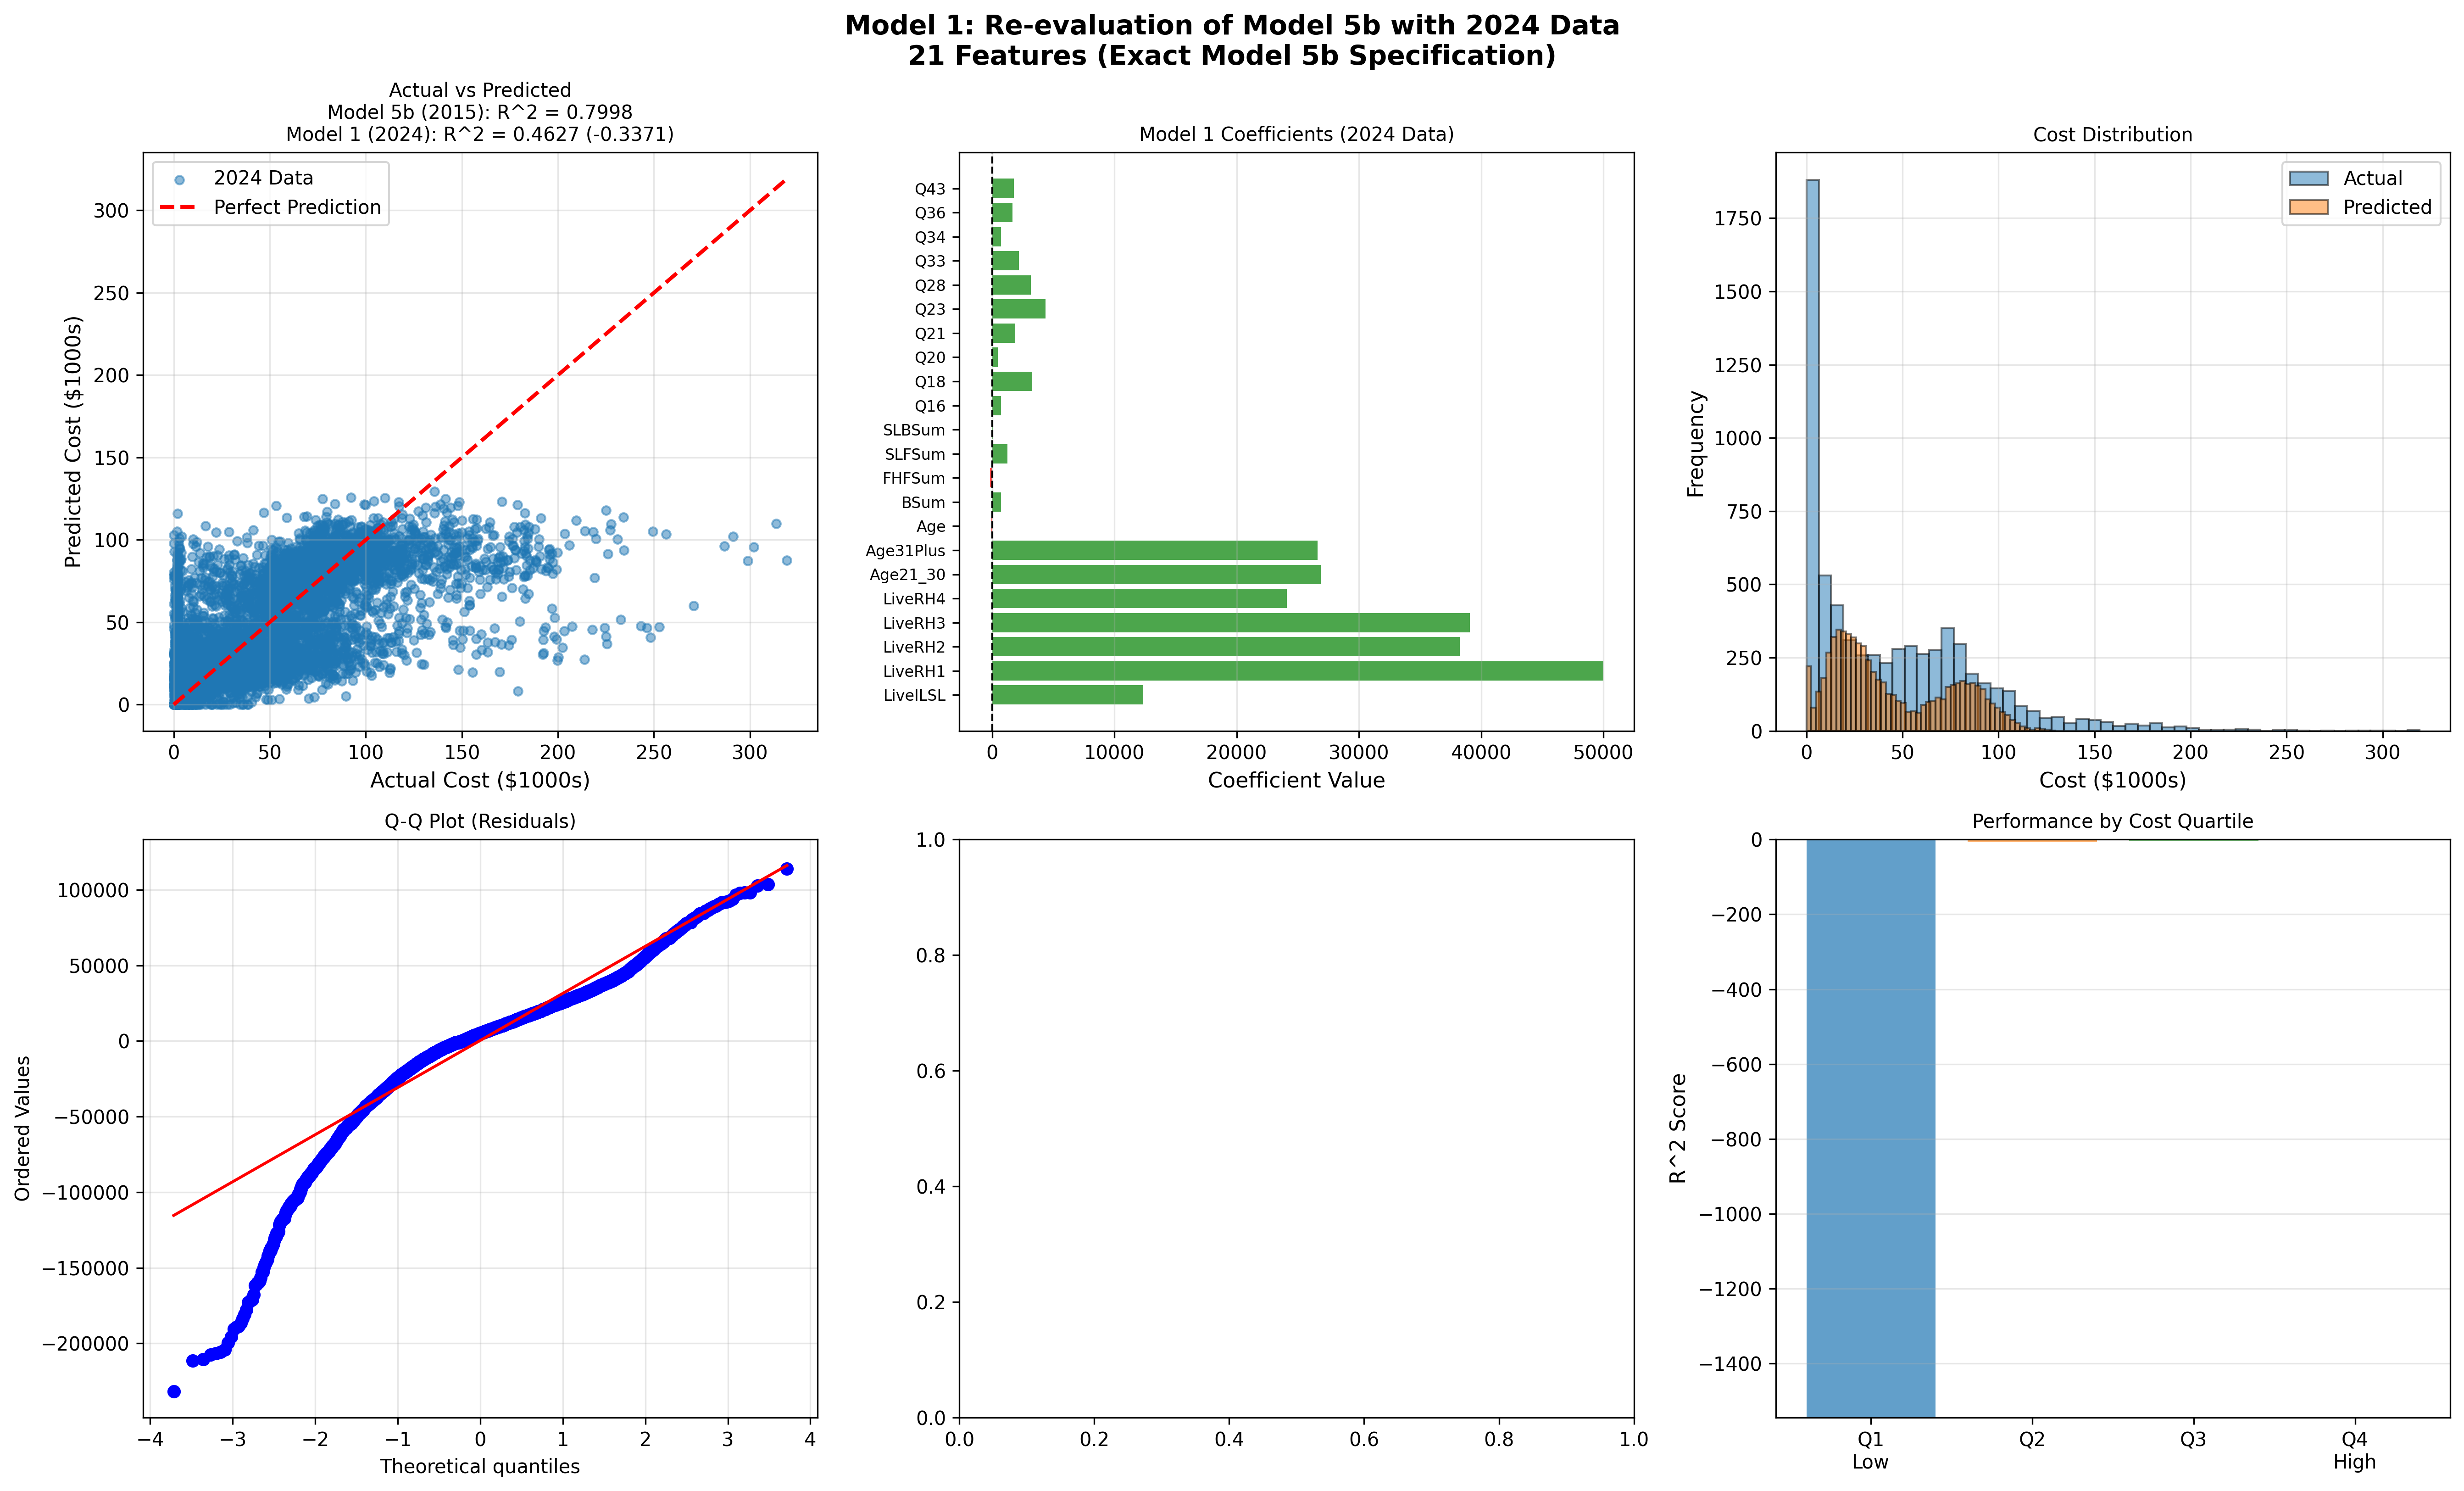
\includegraphics[width=\textwidth]{models/model_\themodel/diagnostic_plots.png}
    \caption{Model Diagnostic Plots --- Shows actual vs.\ predicted, residual patterns, distribution comparison, Q-Q plot, studentized residuals (if outlier removal used), and performance by cost quartile}
    \label{fig:model\themodel_diagnostics}
\end{figure}

\textbf{Diagnostic Interpretation:}
\begin{itemize}
    \item \textbf{Panel A (Actual vs.\ Predicted)}: Points should cluster along the 45° line. Systematic deviations indicate bias in certain cost ranges.
    \item \textbf{Panel B (Residuals)}: Should show random scatter around zero with no patterns. Funnel shapes indicate heteroscedasticity.
    \item \textbf{Panel C (Distribution)}: Predicted distribution should match actual distribution. Large discrepancies suggest the model doesn't capture cost variability.
    \item \textbf{Panel D (Q-Q Plot)}: Tests normality of residuals. Points should follow the diagonal line. Deviations at tails indicate non-normality.
    \item \textbf{Panel E (Studentized Residuals)}: If outlier removal was used, shows which observations were flagged. Should see most points within threshold bounds.
    \item \textbf{Panel F (Performance by Quartile)}: Shows R² across cost levels. Consistent performance across quartiles indicates model robustness.
\end{itemize}

% ============================================
% END OF UNIVERSAL TEMPLATE
% Model-specific content should be added after this point
% ============================================
%
% Now all \M... commands in the template will use Model 1's values
% ============================================
\newcommand{\SetupModelTemplate}[1]{%
    % #1 = Model word (One, Two, Three, ..., Ten)
    
    % ===== Performance Metrics =====
    \expandafter\def\csname MRSquaredTrain\endcsname{\csname Model#1RSquaredTrain\endcsname}%
    \expandafter\def\csname MRSquaredTest\endcsname{\csname Model#1RSquaredTest\endcsname}%
    \expandafter\def\csname MRMSETrain\endcsname{\csname Model#1RMSETrain\endcsname}%
    \expandafter\def\csname MRMSETest\endcsname{\csname Model#1RMSETest\endcsname}%
    \expandafter\def\csname MRMSETrainSqrt\endcsname{\csname Model#1RMSETrainSqrt\endcsname}%
    \expandafter\def\csname MRMSETestSqrt\endcsname{\csname Model#1RMSETestSqrt\endcsname}%    
    \expandafter\def\csname MMAETrain\endcsname{\csname Model#1MAETrain\endcsname}%
    \expandafter\def\csname MMAETest\endcsname{\csname Model#1MAETest\endcsname}%
    \expandafter\def\csname MMAPETrain\endcsname{\csname Model#1MAPETrain\endcsname}%
    \expandafter\def\csname MMAPETest\endcsname{\csname Model#1MAPETest\endcsname}%
    \expandafter\def\csname MCVMean\endcsname{\csname Model#1CVMean\endcsname}%
    \expandafter\def\csname MCVStd\endcsname{\csname Model#1CVStd\endcsname}%
    \expandafter\def\csname MTrainingSamples\endcsname{\csname Model#1TrainingSamples\endcsname}%
    \expandafter\def\csname MTestSamples\endcsname{\csname Model#1TestSamples\endcsname}%
    
    % ===== Accuracy Bands =====
    \expandafter\def\csname MWithinOneK\endcsname{\csname Model#1WithinOneK\endcsname}%
    \expandafter\def\csname MWithinTwoK\endcsname{\csname Model#1WithinTwoK\endcsname}%
    \expandafter\def\csname MWithinFiveK\endcsname{\csname Model#1WithinFiveK\endcsname}%
    \expandafter\def\csname MWithinTenK\endcsname{\csname Model#1WithinTenK\endcsname}%
    \expandafter\def\csname MWithinTwentyK\endcsname{\csname Model#1WithinTwentyK\endcsname}%
    
    % ===== Variance Metrics =====
    \expandafter\def\csname MCVActual\endcsname{\csname Model#1CVActual\endcsname}%
    \expandafter\def\csname MCVPredicted\endcsname{\csname Model#1CVPredicted\endcsname}%
    \expandafter\def\csname MPredictionInterval\endcsname{\csname Model#1PredictionInterval\endcsname}%
    \expandafter\def\csname MBudgetActualCorr\endcsname{\csname Model#1BudgetActualCorr\endcsname}%
    
    % ===== Outlier Metrics =====
    \expandafter\def\csname MOutliersRemoved\endcsname{\csname Model#1OutliersRemoved\endcsname}%
    \expandafter\def\csname MOutlierPct\endcsname{\csname Model#1OutlierPct\endcsname}%
    
    % ===== Subgroup Metrics - Living Settings =====
    \expandafter\def\csname MSubgroupLivingFHRSquared\endcsname{\csname Model#1SubgroupLivingFHRSquared\endcsname}%
    \expandafter\def\csname MSubgroupLivingFHRMSE\endcsname{\csname Model#1SubgroupLivingFHRMSE\endcsname}%
    \expandafter\def\csname MSubgroupLivingFHBias\endcsname{\csname Model#1SubgroupLivingFHBias\endcsname}%
    \expandafter\def\csname MSubgroupLivingFHN\endcsname{\csname Model#1SubgroupLivingFHN\endcsname}%
    
    \expandafter\def\csname MSubgroupLivingILSLRSquared\endcsname{\csname Model#1SubgroupLivingILSLRSquared\endcsname}%
    \expandafter\def\csname MSubgroupLivingILSLRMSE\endcsname{\csname Model#1SubgroupLivingILSLRMSE\endcsname}%
    \expandafter\def\csname MSubgroupLivingILSLBias\endcsname{\csname Model#1SubgroupLivingILSLBias\endcsname}%
    \expandafter\def\csname MSubgroupLivingILSLN\endcsname{\csname Model#1SubgroupLivingILSLN\endcsname}%
    
    \expandafter\def\csname MSubgroupLivingRHOneFourRSquared\endcsname{\csname Model#1SubgroupLivingRHOneFourRSquared\endcsname}%
    \expandafter\def\csname MSubgroupLivingRHOneFourRMSE\endcsname{\csname Model#1SubgroupLivingRHOneFourRMSE\endcsname}%
    \expandafter\def\csname MSubgroupLivingRHOneFourBias\endcsname{\csname Model#1SubgroupLivingRHOneFourBias\endcsname}%
    \expandafter\def\csname MSubgroupLivingRHOneFourN\endcsname{\csname Model#1SubgroupLivingRHOneFourN\endcsname}%
    
    % ===== Subgroup Metrics - Age Groups =====
    \expandafter\def\csname MSubgroupAgeAgeUnderTwentyOneRSquared\endcsname{\csname Model#1SubgroupAgeAgeUnderTwentyOneRSquared\endcsname}%
    \expandafter\def\csname MSubgroupAgeAgeUnderTwentyOneRMSE\endcsname{\csname Model#1SubgroupAgeAgeUnderTwentyOneRMSE\endcsname}%
    \expandafter\def\csname MSubgroupAgeAgeUnderTwentyOneBias\endcsname{\csname Model#1SubgroupAgeAgeUnderTwentyOneBias\endcsname}%
    \expandafter\def\csname MSubgroupAgeAgeUnderTwentyOneN\endcsname{\csname Model#1SubgroupAgeAgeUnderTwentyOneN\endcsname}%
    
    \expandafter\def\csname MSubgroupAgeAgeTwentyOneToThirtyRSquared\endcsname{\csname Model#1SubgroupAgeAgeTwentyOneToThirtyRSquared\endcsname}%
    \expandafter\def\csname MSubgroupAgeAgeTwentyOneToThirtyRMSE\endcsname{\csname Model#1SubgroupAgeAgeTwentyOneToThirtyRMSE\endcsname}%
    \expandafter\def\csname MSubgroupAgeAgeTwentyOneToThirtyBias\endcsname{\csname Model#1SubgroupAgeAgeTwentyOneToThirtyBias\endcsname}%
    \expandafter\def\csname MSubgroupAgeAgeTwentyOneToThirtyN\endcsname{\csname Model#1SubgroupAgeAgeTwentyOneToThirtyN\endcsname}%
    
    \expandafter\def\csname MSubgroupAgeAgeThirtyOnePlusRSquared\endcsname{\csname Model#1SubgroupAgeAgeThirtyOnePlusRSquared\endcsname}%
    \expandafter\def\csname MSubgroupAgeAgeThirtyOnePlusRMSE\endcsname{\csname Model#1SubgroupAgeAgeThirtyOnePlusRMSE\endcsname}%
    \expandafter\def\csname MSubgroupAgeAgeThirtyOnePlusBias\endcsname{\csname Model#1SubgroupAgeAgeThirtyOnePlusBias\endcsname}%
    \expandafter\def\csname MSubgroupAgeAgeThirtyOnePlusN\endcsname{\csname Model#1SubgroupAgeAgeThirtyOnePlusN\endcsname}%
    
    % ===== Subgroup Metrics - Cost Quartiles =====
    \expandafter\def\csname MSubgroupCostQOneLowRSquared\endcsname{\csname Model#1SubgroupCostQOneLowRSquared\endcsname}%
    \expandafter\def\csname MSubgroupCostQOneLowRMSE\endcsname{\csname Model#1SubgroupCostQOneLowRMSE\endcsname}%
    \expandafter\def\csname MSubgroupCostQOneLowBias\endcsname{\csname Model#1SubgroupCostQOneLowBias\endcsname}%
    \expandafter\def\csname MSubgroupCostQOneLowN\endcsname{\csname Model#1SubgroupCostQOneLowN\endcsname}%
    
    \expandafter\def\csname MSubgroupCostQTwoRSquared\endcsname{\csname Model#1SubgroupCostQTwoRSquared\endcsname}%
    \expandafter\def\csname MSubgroupCostQTwoRMSE\endcsname{\csname Model#1SubgroupCostQTwoRMSE\endcsname}%
    \expandafter\def\csname MSubgroupCostQTwoBias\endcsname{\csname Model#1SubgroupCostQTwoBias\endcsname}%
    \expandafter\def\csname MSubgroupCostQTwoN\endcsname{\csname Model#1SubgroupCostQTwoN\endcsname}%
    
    \expandafter\def\csname MSubgroupCostQThreeRSquared\endcsname{\csname Model#1SubgroupCostQThreeRSquared\endcsname}%
    \expandafter\def\csname MSubgroupCostQThreeRMSE\endcsname{\csname Model#1SubgroupCostQThreeRMSE\endcsname}%
    \expandafter\def\csname MSubgroupCostQThreeBias\endcsname{\csname Model#1SubgroupCostQThreeBias\endcsname}%
    \expandafter\def\csname MSubgroupCostQThreeN\endcsname{\csname Model#1SubgroupCostQThreeN\endcsname}%
    
    \expandafter\def\csname MSubgroupCostQFourHighRSquared\endcsname{\csname Model#1SubgroupCostQFourHighRSquared\endcsname}%
    \expandafter\def\csname MSubgroupCostQFourHighRMSE\endcsname{\csname Model#1SubgroupCostQFourHighRMSE\endcsname}%
    \expandafter\def\csname MSubgroupCostQFourHighBias\endcsname{\csname Model#1SubgroupCostQFourHighBias\endcsname}%
    \expandafter\def\csname MSubgroupCostQFourHighN\endcsname{\csname Model#1SubgroupCostQFourHighN\endcsname}%
    
    % ===== Population Scenarios =====
    % Current Baseline
    \expandafter\def\csname MPopcurrentbaselineClients\endcsname{\csname Model#1PopcurrentbaselineClients\endcsname}%
    \expandafter\def\csname MPopcurrentbaselineAvgAlloc\endcsname{\csname Model#1PopcurrentbaselineAvgAlloc\endcsname}%
    \expandafter\def\csname MPopcurrentbaselineWaitlistChange\endcsname{\csname Model#1PopcurrentbaselineWaitlistChange\endcsname}%
    \expandafter\def\csname MPopcurrentbaselineWaitlistPct\endcsname{\csname Model#1PopcurrentbaselineWaitlistPct\endcsname}%
    
    % Model Balanced
    \expandafter\def\csname MPopmodelbalancedClients\endcsname{\csname Model#1PopmodelbalancedClients\endcsname}%
    \expandafter\def\csname MPopmodelbalancedAvgAlloc\endcsname{\csname Model#1PopmodelbalancedAvgAlloc\endcsname}%
    \expandafter\def\csname MPopmodelbalancedWaitlistChange\endcsname{\csname Model#1PopmodelbalancedWaitlistChange\endcsname}%
    \expandafter\def\csname MPopmodelbalancedWaitlistPct\endcsname{\csname Model#1PopmodelbalancedWaitlistPct\endcsname}%
    
    % Model Efficiency
    \expandafter\def\csname MPopmodelefficiencyClients\endcsname{\csname Model#1PopmodelefficiencyClients\endcsname}%
    \expandafter\def\csname MPopmodelefficiencyAvgAlloc\endcsname{\csname Model#1PopmodelefficiencyAvgAlloc\endcsname}%
    \expandafter\def\csname MPopmodelefficiencyWaitlistChange\endcsname{\csname Model#1PopmodelefficiencyWaitlistChange\endcsname}%
    \expandafter\def\csname MPopmodelefficiencyWaitlistPct\endcsname{\csname Model#1PopmodelefficiencyWaitlistPct\endcsname}%
    
    % Category Focused
    \expandafter\def\csname MPopcategoryfocusedClients\endcsname{\csname Model#1PopcategoryfocusedClients\endcsname}%
    \expandafter\def\csname MPopcategoryfocusedAvgAlloc\endcsname{\csname Model#1PopcategoryfocusedAvgAlloc\endcsname}%
    \expandafter\def\csname MPopcategoryfocusedWaitlistChange\endcsname{\csname Model#1PopcategoryfocusedWaitlistChange\endcsname}%
    \expandafter\def\csname MPopcategoryfocusedWaitlistPct\endcsname{\csname Model#1PopcategoryfocusedWaitlistPct\endcsname}%
}

